\documentclass[10pt,a4paper]{article}
\usepackage[utf8]{inputenc}
\usepackage{amsmath}
\usepackage{amsfonts}
\usepackage{amssymb}
\usepackage{graphicx}


\usepackage[usenames,dvipsnames]{xcolor}
\newcommand{\Wilma}[1]{\textcolor{Magenta}{#1}}
\newcommand{\HW}[1]{\textcolor{Green}{#1}}
\newcommand{\Jo}[1]{\textcolor{Cyan}{#1}}
\newcommand{\Elena}[1]{\textcolor{Orange}{#1}}
\newcommand{\Answer}[1]{\textcolor{Gray}{#1}}

\usepackage{soul}

\begin{document}
\section*{Reviewer's Comments on "Action-based Dynamical Modeling for the Milky Way Disk: The Influence of Spiral Arms" (14. November 2016) \& Answers (18. February 2016)}

\paragraph{Summary of the paper:} The article is a follow up of Paper I, which presented a method (RoadMapping) to constrain the MW potential from data. In Paper I, mock data were obtained, assuming
the potential is axisymmetric, which was a simplistic approximation. In this second
paper, the mock data are obtained from N-body simulations, showing spiral arms.

\paragraph{Main concerns, Aspect 1 \& 2:} (1) However, there is no bar in the simulations, which again is a very simplistic approximation.  (2) Also the spiral structure is faint, and uncontrasted with respect to
the total potential.

\Answer{On (1): That our simulation does not have a bar is indeed a limitation of the methodology used in this paper. We made that clear in the paper, and now mention it in the abstract, in the introduction, in a new section 2.5, which compares the simulation and the MW, and we also moved the paragraph on the bar in the discussion to a more prominent position in Section 5.5. Ultimately we are not trying to analyze the most realistic non-axisymmetric MW simulation, but rather one with very strong spiral arms.}

\Answer{On (2): The referee's second concern, that the spiral structure is too faint, is however not the case. We will discuss this in more detail below.}
 
\paragraph{Summary of the paper (continued):} The authors have done a thorough and very detailed analysis of the mock data, varying the center of the volume (Sun at the inter-arm, or on an arm, etc..), and
checked how much the volume of data considered changes the results. This is very
useful to prepare the exploitation of Gaia data.

\paragraph{Aspect 2: Amplitude of spiral arms (continued):} The present study concludes that RoadMapping is still relatively valid when considering spiral structure, however this referee is not quite convinced that this
will apply to the MW, since the N-body models considered here are so axisymmetric,
and the spiral structure amplitude so negligible. In the real MW world, the contrast
of spiral arms and bars will be much higher in the potential, and will perturb much
more the orbits.  

\Answer{We do not think that it is the case that the spiral arms in this simulation are much weaker than in the MW.}

\Answer{(a) Figure 5 in the paper compares the stellar data with an axisymmetric best-fit model and it is very obvious that there are very strong non-axisymmetries and an excess of stars with $v_R\sim 50~\text{km/s}$ due to the spiral arms. Non-axisymmetric motions in the MW are around $10-20~\text{km/s}$.}

\Answer{(b) Figure 2a in the paper demonstrates that the surface density variations with $\phi$ due to the spiral arms in the disk only are very strong, especially around $R=5~\text{kpc}$. (Figure 2 is a new plot we included in the paper to make this very clear.) Spiral arms around this radius affect almost all of our survey volumes, also those that are centered at $R=8~\text{kpc}$ for $r_\text{max}\gtrsim2~\text{kpc}$.}

\Answer{(c) Figure 10 in the paper shows the total (incl. dark matter) circular velocity curve and radial surface density profile within a small $\Delta \phi$ wedge. The spiral arms are therefore strong perturbations also in the total potential.}

\Answer{(d) Figure 7 in the paper shows that the total gravitational force perturbations due to the spiral arms with respect to an axisymmetric model are $\sim30\%$.}

\paragraph{Aspect 3: dark matter fraction:} Indeed, the model considered here is dominated by dark matter (stellar disk mass fraction of 4\%, also stabilized by a spherical bulge of mass 25\% of the stellar disk mass). The amplitude of the spiral arms obtained certainly brings a negligible
perturbation on the total gravitational potential of the galaxy model. In the
realistic MW, the dark matter fraction within the solar radius has been established
to be much less (the MW inside the solar radius is dominated by baryons, e.g. Barros
et al 2016 A\&A 593, A108 and references therein.). The dominance of baryons and the
much higher gas fraction make the disk much more self-gravitating and unstable, and
the bar amplitude is non-negligible, as well as the strong spiral arms associated.

\Answer{The stellar disk fraction of 4\% is only the fraction of the \emph{total} mass of the dark matter halo. Locally the disk dominates over dark halo and bulge, especially between $R=3-7~\text{kpc}$. The mass enclosed in $2.2R_\text{s}$ is 50\% (see Section 2.1 and D'Onghia et al. 2013). The rotational support at $2.2R_s$ is $\sim47\%$ as shown in Figure \ref{fig:rot_support} below for the reference potential \texttt{DEHH-Pot}. The upper panel of Figure \ref{fig:rot_support}, which shows the decomposition of the rotation curve of the \texttt{DEHH-Pot}, was also included in the paper as Figure 3 to also make this clear to the reader.}

\Answer{In the new Section 2.5 in the paper we discuss how the mass budgets of the simulation and of the MW compare with each other. Given the uncertainty in our knowledge about the MW, the simulation's mass components (including bulge and halo) are of a similar order of magnitude than those in the MW.}

\Answer{We also compare the simulation with the MW models from Barros et al. (2016) and find that one of their two MW models is qualitatively not too different to our simulation.}

\Answer{We do not worry about the gas, because given that the gravitational perturbations in this simulation are quite strong, the combined gravitational perturbations of stars and gas in the MW should be possible to deal with by RoadMapping.}

\Answer{The only major deviation from the MW is indeed, that there is no bar (see above).}

%====================
\begin{figure}[!htbp]
\centering
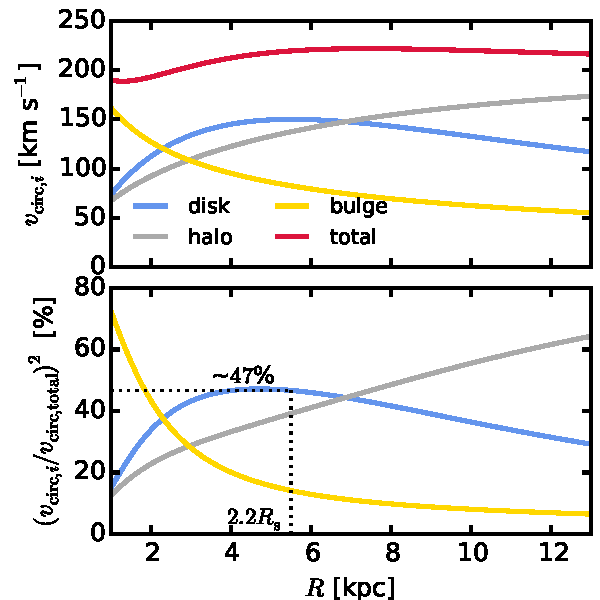
\includegraphics[width=0.7\columnwidth]{fig/plot_vcirc_decomposed.pdf}
\caption{\Answer{Circular velocity curve and fractional contribution to the radial force (rotational support) of the disk, halo and bulge components of the \texttt{DEHH-Pot}, the symmetrized best fit to the $N$-body simulation. This demonstrates that the simulation is a disk-dominated spiral galaxy.}}
\label{fig:rot_support}
\end{figure}
%====================

\paragraph{Aspect 2: Amplitude of spiral arms (continued):} The model considered here, almost axisymmetric (the contrast of the spiral structure is in its large majority less than or equal to 10\% in stellar surface density, as shown in Figure 2),  is therefore very far from the reality of the MW, and can be highly deceiving for the MW results to come.

\Answer{The referee is right that the Figure 4 in the paper (previously Figure 2) shows that outside of $R\sim9-10~\text{kpc}$ the majority of the area has a spiral contrast of less than 10\%. However, even further out there are still some perturbations of up to 50\%. Inside of $R\sim8~\text{kpc}$ we have extremely strong perturbations of 100\% or more, as can be seen both in Figure 2a and 4 in the paper. As there is always an excess of stars in the data sets which come from within spiral overdensities and---due to the exponential density profile---from smaller radii where the perturbations are stronger, it does not give the modelling an unfair advantage, that there are larger areas outside of $R\sim9-10~\text{kpc}$ which have less strong perturbations and in general less stars.}

\Answer{Considering the strength of the spiral arms in the MW, we have also added a comment in Section 2.5 in the paper.}

\paragraph{Aspect 4: Conservation of actions} The fact that the DF is still expressed in terms of integrals of motion, which should not be any more conserved, is a questionable issue.

\Answer{Actions in an axisymmetric potential are integrals of motions and according to the Jeans Theorem any steady-state distribution function solution to the Boltzmann equation becomes $DF(\vec{x},\vec{v},t) \longrightarrow DF(\vec{J})$. In an axisymmetric potential superimposed with non-axisymmetric perturbations, actions are indeed not fully conserved anymore. It is however still possible to estimate the local current actions (using an axisymmetric approximation to the potential) and treat $(\vec{J},\vec{\theta})$ simply as phase-space coordinates analogous to $(\vec{x},\vec{v})$. It is interesting to test, if using the $qDF(\vec{J})$ locally as model for the true $DF(\vec{x},\vec{v},t)\approx DF(\vec{J},\vec{\theta},t)$ could still tell us something about the true potential. This is one of the aspects of action-based modelling we wanted to test in this study---and which we found to be indeed the case. To make this motivation more clear in the paper, we have included a paragraph in the introduction and another one in Section 3.2 about the distribution function model.}

\paragraph{Aspect 5: Radial migration and MAP concept:} Moreover, we know that spiral structure will trigger radial migration of stars, the
more so that there velocity dispersion is small. So for a given stellar population,
with a given metal abundance (and alpha/FE ratio), we expect that a dispersion will
occur in orbits, and the MAP concept will no longer be valid. 

\Answer{The simulation at hand does not have any chemical abundances. We treat the whole disk as one single MAP (be it mono-abundance or mono-age population and motivate in Section 3.2 why we think, given the setup of the disk, that the qDF might be a good model for the overall average particle distribution. If this assumption is still valid after some time, when radial migration has re-distributed the stars, was one of the aspects to investigate in this work. Surprisingly the fits still gave plausible results.}

\Answer{Considering MAPs in the MW: The interesting property of MAPs, which is that their distribution and kinematics appear to be described by simple functions was fully perceived from and only motivated by the SEGUE G-dwarf data in the MW (Bovy et al. 2012a,b,c, Ting et al. 2013, Bovy et al. 2016). It is a question that is not fully answered yet how the inside-out growth and subsequent secular evolution of the MW, including radial migration, caused the build-up of such a disk composed of MAPs with simple structure. The interesting question is therefore not, how does the MAP concept work in the presence of radial migration, but rather, how did radial migration lead to the fact that MAPs appear to be a useful concept when modelling the MW.}

\Answer{Bovy et al. (2016) suggest, that the qDF might not be flexible enough to describe low [$\alpha$/Fe] MAPs. But we plan in the future for the application to MW data to incorporate more flexible radial profiles in the qDF and also allow for flaring.}

\paragraph{Question 1: Corotation of spiral arms} About this problem, it will be also useful to mention where is the corotation of the
spiral in the N-body model, is it near the Sun radius?

\Answer{This would be indeed good to know. Unfortunately this is not easy to determine for this N-body simulation. The spiral arms in this simulation are transient. And we do not have enough simulation snapshots to determine the patter speed of these transient spiral arms. We hope however, that this is not a huge issue, given that we successfully analyse data drawn from anywhere between $R=1~\text{kpc}$ and $R=13~\text{kpc}$ and survey volumes of different sizes and at different positions. If the co-rotation would affect the modelling strongly, we would have noticed.} \hl{Elena, is there anything else, we can say about that?}

\paragraph{Question 2: Thick disk:} Another simplification of the N-body model is that there is no thick disk, while in
the MW, there is one which is about comparable mass to the thin disk. How will the
presence of this other components change the study of the orbits, and derivation of
the potential?

\Answer{Incorporating the thick disk in an application to MW data will be absolutely no problem for RoadMapping. There are two aspects in the modelling: The distribution function and the potential model. (a) In the potential model we can simply include the thick disk as an additional component, for example, having two exponential or Miyamoto-Nagai disk components of different thickness and scale length. (If we want, we could add a third disk for the gas mass). The only problem would be the number of free model parameters, but this is a purely computational issue. (b) In the distribution of stars the thick disk is automatically taken care of. By separating the data first into MAPs in [Fe/H] and [$\alpha$/Fe] the thick disk stars will fall into the high-$\alpha$ MAPs and will be independently modelled. In that way the different spatial distribution and higher velocity dispersion is directly taken care of.}

\Answer{Modelling the thick disk stars might be even more straight forward than modelling thin disk stars: They have a simpler phase-space structure, that can be captured by the qDF in its current form (Bovy et al. 2016), and due to the high velocity dispersion they are also less affected by spiral perturbations.}

\Answer{We mention all of this also briefly in Section 2.5 in the paper.}

\Answer{The reason why we picked a simulation with a very cold disk, was to have a very strong response of the stars to gravitational perturbations.}

\paragraph{Aspect 6: No spiral arms outside of the solar radius.} Another issue is that the model considered has spiral arms only within the solar
radius, and is axisymmetric in the outer parts. Not surprisingly, there are big
departures from the true DF inside the solar radii, and less outside, as shown in
Figure 3. This will not be the case for a realistic MW model. 

\Answer{The referee is right that the spiral arms in the simulation outside of the solar radius are relatively weak. If this is the case in the MW as well, or not, is not fully known.}

\Answer{Still, even the perturbations in this simulation outside of $R=8~\text{kpc}$ are not completely negligible. As can be seen in Figure 4a in the paper, there are still spiral perturbations of up to $\sim30-50\%$ out to $R=9-10~\text{kpc}$ in stellar surface density. In Figure 5a (previously Figure 3a) in the paper the departures from the true DF outside of $R=8~\text{kpc}$ still have a residual significance of 2-3 sigma. In the 1D spatial histograms the impression that there were no spiral arms outside of the solar radius is strengthened by averaging over the other two spatial coordinates.}

\Answer{We made sure to also investigate data sets that do not come from regions that are partly smooth; that's why we also investigated data from survey volumes around $R=5~\text{kpc}$.}

\Answer{Figures 9-11 in the paper show the radial extent of the survey volumes and mark the radial bins in which the majority of stars within a given data set is located with a brighter shade in color. These regions with an excess of stars appeared to drive the fit. And as can be seen the huge majority of these regions is located inside $R=8~\text{kpc}$, where the spiral arms are strong.}

\paragraph{Aspect 2 \& 3 (continued):} p.19 in the conclusion: the authors conclude that their model has "has stronger spiral arms than we expect in the MW", which is not true, given the dominance of
the dark matter

\Answer{Typical fluctuations due to spiral arms in the MW are somewhere of the order of $10-20~\text{km s}^{-1}$ (e.g., Reid et al. 2014, Siebert et al. 2012). We measure similar or stronger velocity perturbations in our simulation (see Figure 5c in the paper). (We mention this in Section 2.5.) Also, the dark matter halo is not as dominant (see above). We therefore still think that the spiral arm strength is at least comparable to that in the MW.}

\paragraph{Aspect 7: Number of spiral arms} It should also be recalled that in the MW when the true stellar component is mapped
in the NIR, the number of spiral arms turns out to be 2 only, while it is more 4
arms when Halpha and young stars are considered. This means that gas and star
formation are participating to harmonics and branching, but the basic stellar
structure is 2-armed. This will modify the conclusion, since the importance of
spiral arms in the stellar structure will be higher.

\Answer{This is a good point, thank you. We have included a paragraph on the suspected number of spiral arms in the MW in Section 2.5 of the paper. In the conclusion, in Section 5.4, we have also mentioned that a lower number of spiral arms would require larger survey volumes to be able to successfully average over several spiral arms.}

\Answer{As can be seen in Figure 2b in the paper, the simulation is a four-armed spiral between $R=4-7~\text{kpc}$, a two-armed spiral inside of this and more flocculent in the outer regions. Especially the survey volumes centered at $R=5~\text{kpc}$ deal therefore with spiral arm situations that could be similar to the MW. But also for small survey volumes centered at this radius we got some good average results.}

\paragraph{Task 1: Callibrating the method using smooth data.} There is also some issue which is striking in the paper, is that the departures from
the model are very high, when looking at Fig 3, 6 or even 11. And the reader wonders
how much is due already to the N-body model without spiral arms. Therefore it might
be interesting to calibrate the method, using the snapshot T=0 (or close to 0), the
initial axisymmetric model without spiral arms, and apply RoadMapping to understand
the  influence of the basic model. This might not be a long task, only providing a
test, or a Figure, but certainly will help to understand the high discrepancy
between derived results and the model.

\Answer{This was a very good idea and we have performed this callibration test and included a section on it in the paper (Section 4.1.4).}

\Answer{The problem with this test was, however, that the initial snapshot uses a velocity setup of the disk, that uses simply triaxial Gaussians for the velocity dispersion. This is not completely physical (especially not for the $v_T$ velocities) and also not self-consistent and we expect the modelling to be biased by this. The simulation develops immediately spiral arms, so there was no other useful snapshot we could perform the callibration on.}

\Answer{Given that, the fit was still quite successful. In Figures 2 and 3 below we compare the true and best fit distribution of stars in this initial snapshot. Except of $v_T$, the fit is quite good and will convince the referee that the qDF is indeed a good model for the axisymmetric set-up of the disk. The deviations in Figure 5 in the paper (previously Figure 3) are therefore fully due to the spiral arms.}

\Answer{Figure 7 in the paper (previously Figure 6) shows strong deviations in the gravitational forces in and around the spiral arms between the model and the data, because the axisymmetric model cannot reproduce the spiral arms. The model is however able to find a good average model, even though the perturbations due to the spiral arms are up to $\sim30\%$.}

\Answer{Figure 12 in the paper (previously Figure 11) shows that we only recover the true potential parameters for large survey volumes. One of the key results of the paper is, however, that we always recover the gravitational forces at the average position of the data. For a small volume dominated by a spiral arm we do not expect the overall potential to be recovered, but to get a local estimate of the potential. This leads to deviations in the recovered parameters for small volumes as compared to the overall true parameters. This does not mean, that the fit is bad, quite on the contrary, as we explain in detail in Sections 4.2.2-4.2.4.}

%====================
\begin{figure}[!htbp]
\centering
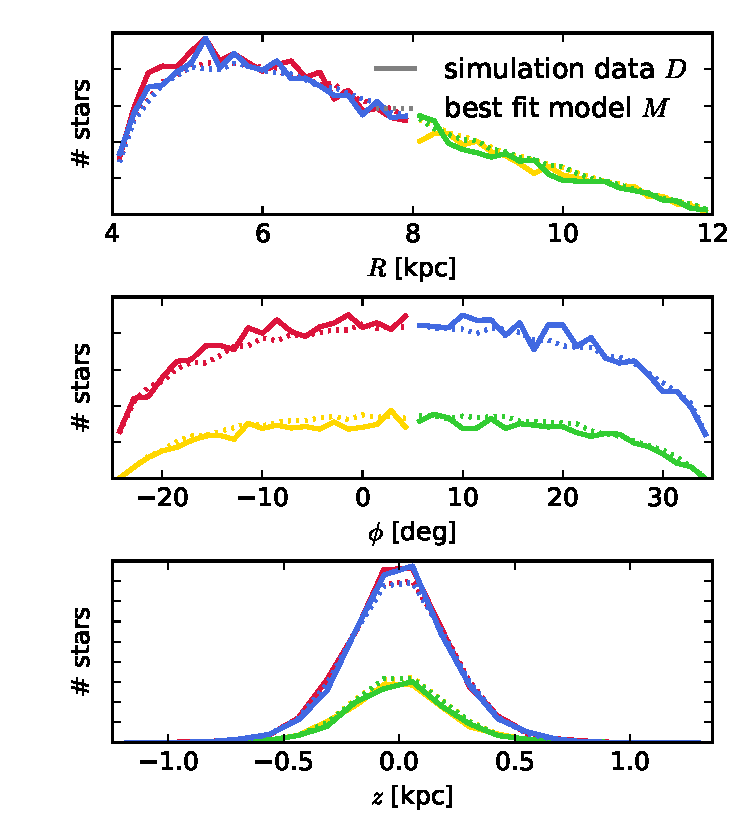
\includegraphics[width=0.7\columnwidth]{fig/MNdHHinit_4kpc8Spiral_a_test1_data_bestfit_residuals_3b.pdf}
\caption{\Answer{Comparison of the 1D spatial distribution of particles drawn from the initial axisymmetric simulation snapshot (data $D$, solid line) with the best fit RoadMapping model (model $M$, dotted line). The data was drawn from within a survey volume with $r_\text{max}=4~\text{kpc}$ around the position \texttt{S8}, $(R_0,\phi_0,z_0)=(8~\text{kpc},5~\text{deg},0~\text{kpc})$. The agreement between data and model is very good.}}
\label{fig:MNinit_spatial}
\end{figure}
%====================

%====================
\begin{figure}[!htbp]
\centering
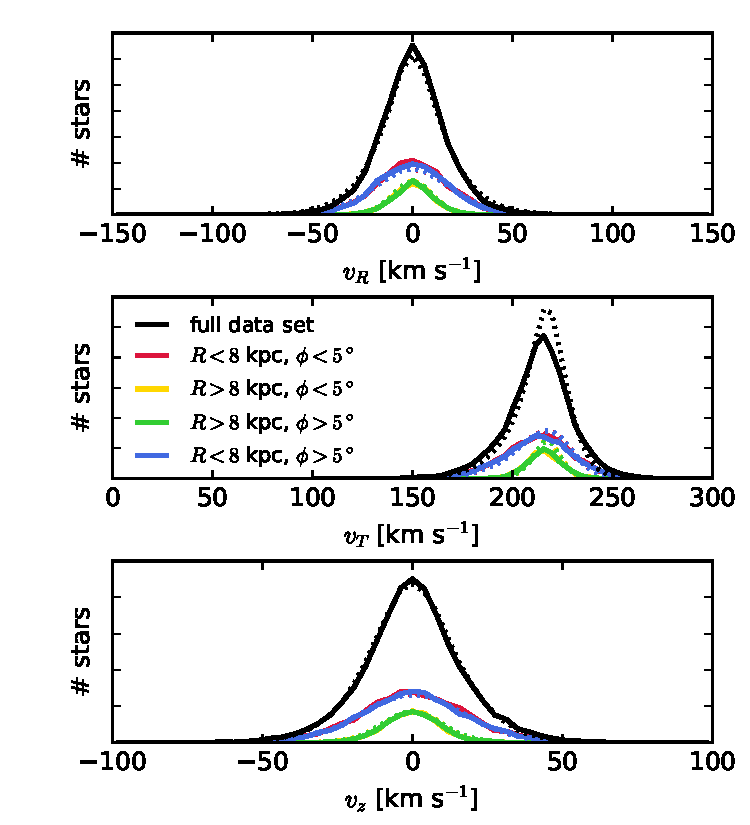
\includegraphics[width=0.7\columnwidth]{fig/MNdHHinit_4kpc8Spiral_a_test1_data_bestfit_residuals_3c.pdf}
\caption{\Answer{Same as Figure \ref{fig:MNinit_spatial}, but for the velocity distribution. Except of $v_T$ the fit is also good. The model predicts more asymmetric drift in $v_T$ as compared to the data. The reason is that the initial velocity distribution in the simulation is set up following a triaxial Gaussian velocity dispersion.}}
\end{figure}
%====================


\paragraph{Comment regarding the software policy:}

Per the new AAS software policy, http://journals.aas.org/policy/software.html, the
authors should use AASTeX v6.1 for the revised manuscript to highlight the code they
used with the new {\textbackslash}software command, e.g.

{\textbackslash}software{GADGET-3 (Springel et al. 2005), galpy (Bovy 2008), emcee (Foreman-Mackey
et al. 2013)}

\hl{Forgot to do that---will deal with it next week.}

\paragraph{\Answer{Additional changes in the paper to make it more readable and easier to understand:}}
\begin{itemize}
\item \Answer{We removed several panels in plots that were nice to have, but which appeared to draw attention away from the key plots and messages. We have indicated in the paper where this happened.}
\item \Answer{We have completely re-structured Sections 4.2.4-4.2.6, to have one section per diagnostic and result, and not mix them and the plots concerning them. It should now be much easier to understand.}
\item \Answer{We have slightly rephrased some sentences to make them clearer. Legends and labels in plots were made larger.}
\end{itemize}

\end{document}